% 2006 安徽卷理 Q16；立方体置于平面示意图，虚线为遮挡棱。
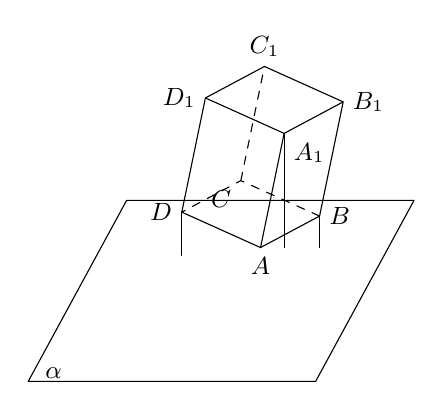
\begin{tikzpicture}[line cap=round,line join=round,font=\small]
  \coordinate (A)  at (1.25,0.35);
  \coordinate (B)  at (2.00,0.75);
  \coordinate (C)  at (1.00,1.20);
  \coordinate (D)  at (0.25,0.80);
  \coordinate (A1) at (1.55,1.80);
  \coordinate (B1) at (2.30,2.20);
  \coordinate (C1) at (1.30,2.65);
  \coordinate (D1) at (0.55,2.25);

  % 平面 α：A 位于其上，边界按源图作透视示意。
  \draw (-0.45,0.95)--(3.20,0.95)--(1.95,-1.35)--(-1.70,-1.35)--cycle;

  % 立方体可见棱与遮挡棱。
  \draw (D)--(A)--(B);
  \draw[dashed] (B)--(C)--(D);
  \draw (D)--(D1) (A)--(A1) (B)--(B1);
  \draw[dashed] (C)--(C1);
  \draw (D1)--(C1)--(B1)--(A1)--cycle;

  % 相邻顶点到平面 α 的距离线，仅作源图中的位置示意，不标尺寸。
  \draw[thin] (D)--(0.25,0.25);
  \draw[thin] (B)--(2.00,0.35);
  \draw[thin] (A1)--(1.55,0.35);

  \node[below] at (A) {$A$};
  \node[right] at (B) {$B$};
  \node[below left] at (C) {$C$};
  \node[left] at (D) {$D$};
  \node[below right] at (A1) {$A_1$};
  \node[right] at (B1) {$B_1$};
  \node[above] at (C1) {$C_1$};
  \node[left] at (D1) {$D_1$};
  \node[below left] at (-1.15,-1.05) {$\alpha$};
\end{tikzpicture}
